\documentclass[a4paper, 10pt]{article}
\usepackage[T1]{fontenc}
\usepackage[utf8]{inputenc}
\usepackage[english]{babel}
\usepackage{graphicx}
\usepackage{caption}


\begin{document}
\begin{figure}
\begin{minipage}{.4\textwidth}
\centering
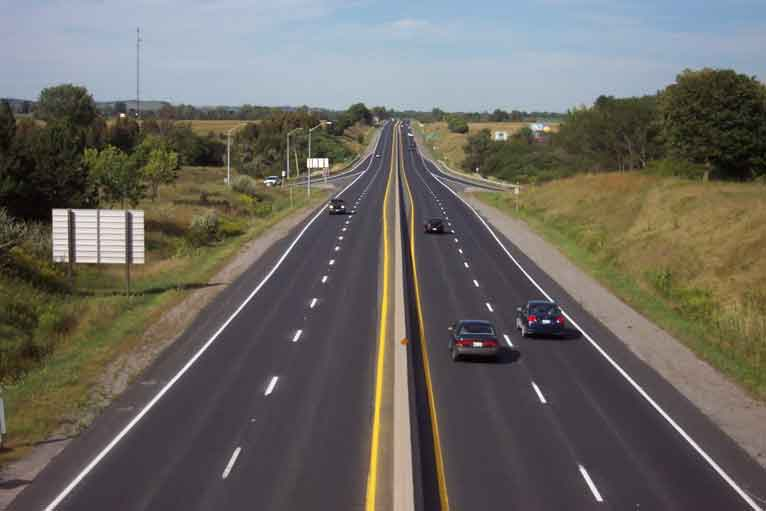
\includegraphics[scale=0.14]{images/highway.jpg}
\captionof{figure}{Image originelle d'autoroute}
\end{minipage}%
\begin{minipage}{.4\textwidth}
\centering
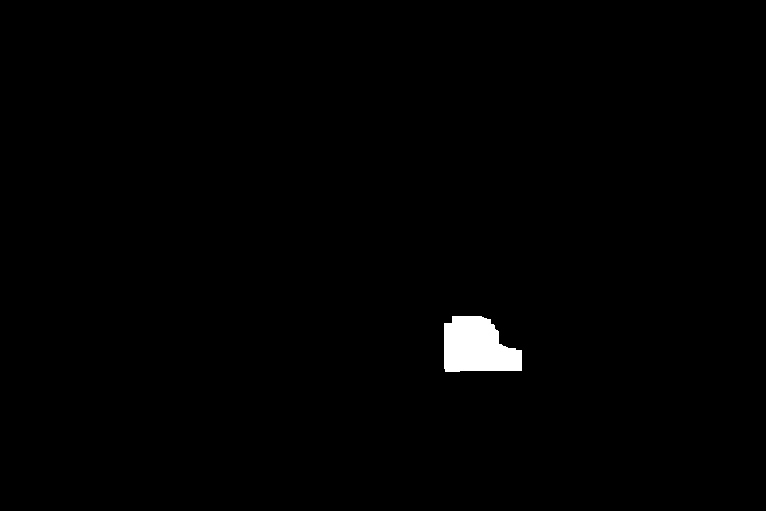
\includegraphics[scale=0.14]{highway-mask.png}
\captionof{figure}{Masque appliqué}
\end{minipage}%
\begin{minipage}{.4\textwidth}
\centering
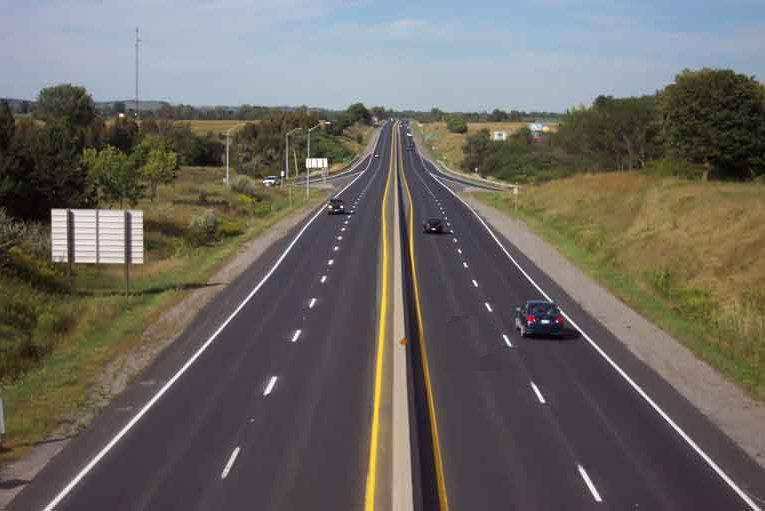
\includegraphics[scale=0.14]{inpainted_highway17.png}
\captionof{figure}{Résultat d'Inpainting avec p=17}
\end{minipage}%

\end{figure}
\begin{figure}
\begin{minipage}{.4\textwidth}
\centering
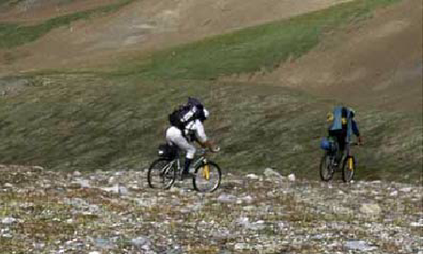
\includegraphics[scale=0.25]{images/bike.png}
\captionof{figure}{Image originelle de vélos}
\end{minipage}%
\begin{minipage}{.4\textwidth}
\centering
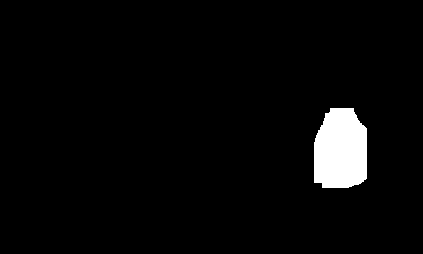
\includegraphics[scale=0.25]{bike_mask17.png}
\captionof{figure}{Masque appliqué}
\end{minipage}%
\begin{minipage}{.4\textwidth}
\centering
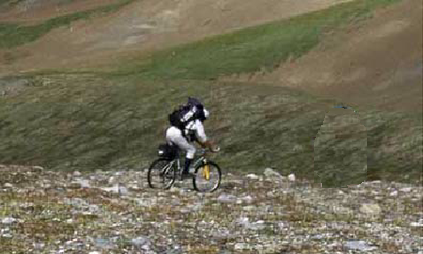
\includegraphics[scale=0.25]{inpainted_bike17.png}
\captionof{figure}{Résultat d'Inpainting avec p=17}
\end{minipage}%

\end{figure}


\begin{figure}
\begin{minipage}{.4\textwidth}
\centering
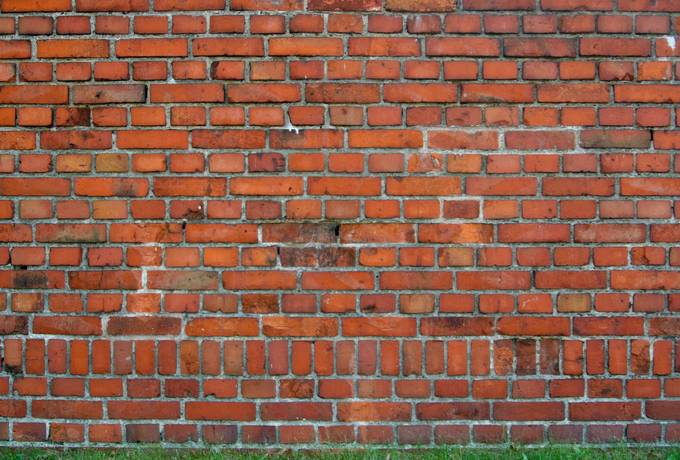
\includegraphics[scale=0.15]{images/wall3.jpg}
\captionof{figure}{Image originelle de mur}
\end{minipage}%
\begin{minipage}{.4\textwidth}
\centering
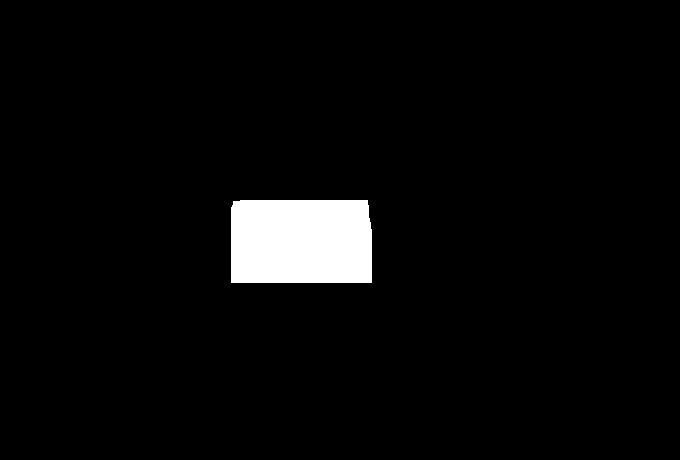
\includegraphics[scale=0.15]{mask_wall3_29.png}
\captionof{figure}{Masque appliqué}
\end{minipage}%
\begin{minipage}{.4\textwidth}
\centering
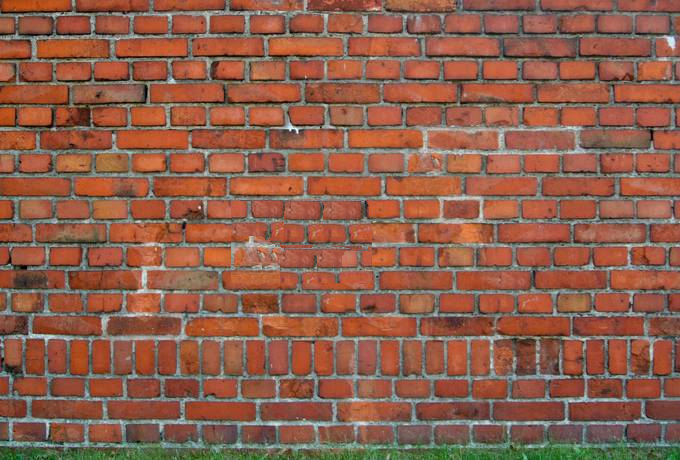
\includegraphics[scale=0.15]{wall3_inpainted29.png}
\captionof{figure}{Résultat d'Inpainting avec p=29}
\end{minipage}%
\end{figure}

\begin{figure}
\begin{minipage}{.4\textwidth}
\centering
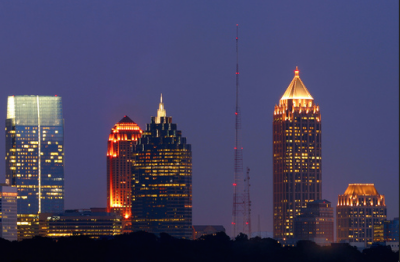
\includegraphics[scale=0.25]{images/skyline.png}
\captionof{figure}{Image originelle de buildings}
\end{minipage}%
\begin{minipage}{.4\textwidth}
\centering
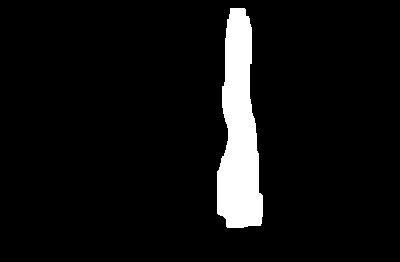
\includegraphics[scale=0.25]{skyline-mask.png}
\captionof{figure}{Masque appliqué}
\end{minipage}%
\begin{minipage}{.4\textwidth}
\centering
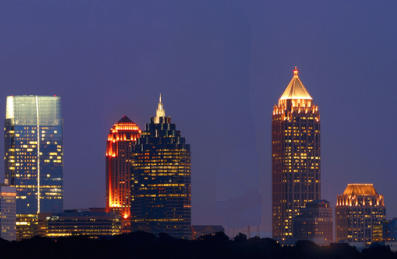
\includegraphics[scale=0.25]{inpainted_skyline17.png}
\captionof{figure}{Résultat d'Inpainting avec p=17}
\end{minipage}%
\end{figure}

\begin{figure}
\begin{minipage}{.4\textwidth}
\centering
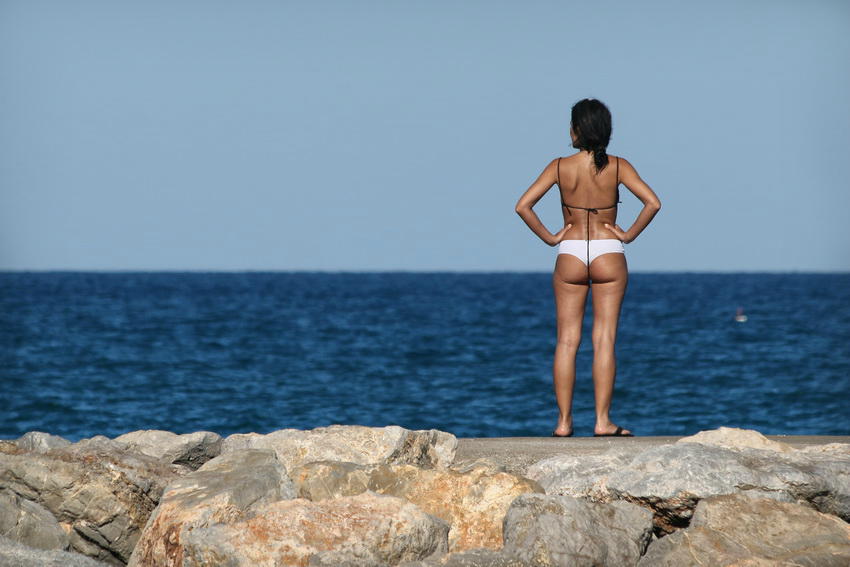
\includegraphics[scale=0.15]{images/women.png}
\captionof{figure}{Image originelle de femme devant la mer}
\end{minipage}%
\begin{minipage}{.4\textwidth}
\centering
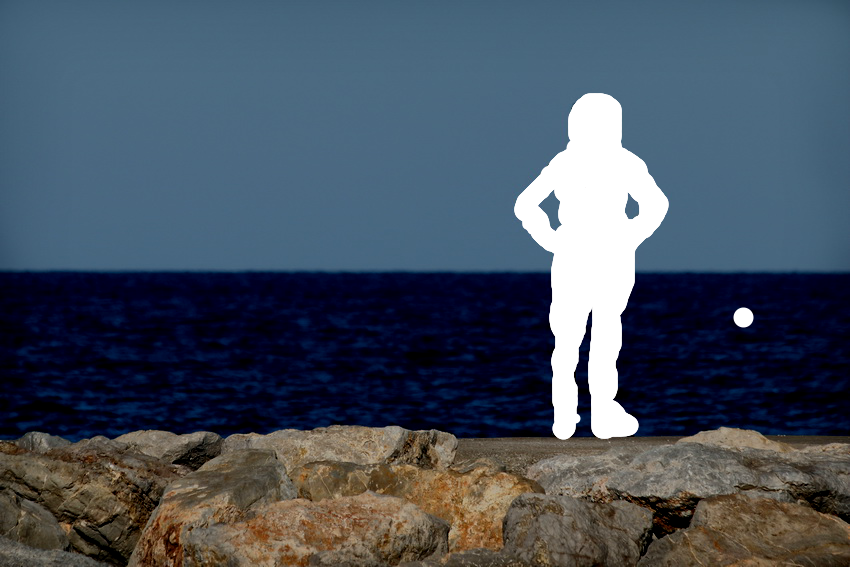
\includegraphics[scale=0.15]{images/women-mask.png}
\captionof{figure}{Masque appliqué}
\end{minipage}%
\begin{minipage}{.4\textwidth}
\centering
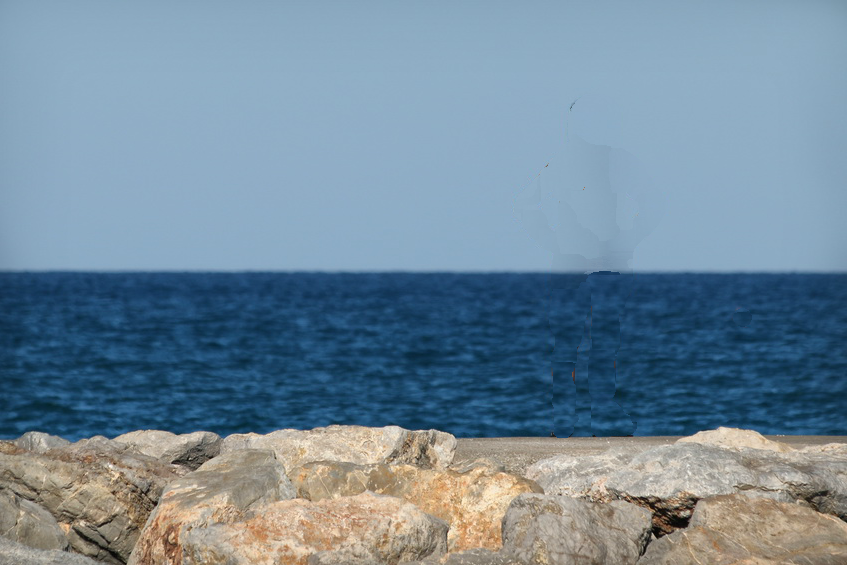
\includegraphics[scale=0.15]{inpainted_women27.png}
\captionof{figure}{Résultat d'Inpainting avec p=27}
\end{minipage}%
\end{figure}

\begin{figure}
\begin{minipage}{.4\textwidth}
\centering
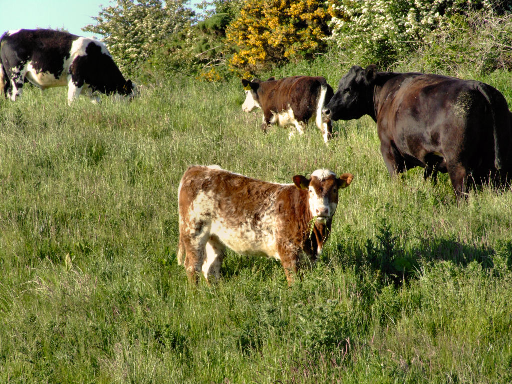
\includegraphics[scale=0.25]{images/cow.png}
\captionof{figure}{Image originelle de vaches}
\end{minipage}%
\begin{minipage}{.4\textwidth}
\centering
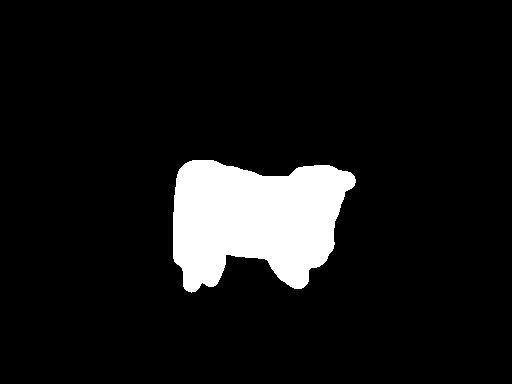
\includegraphics[scale=0.25]{images/cow-mask.png}
\captionof{figure}{Masque appliqué}
\end{minipage}%
\begin{minipage}{.4\textwidth}
\centering
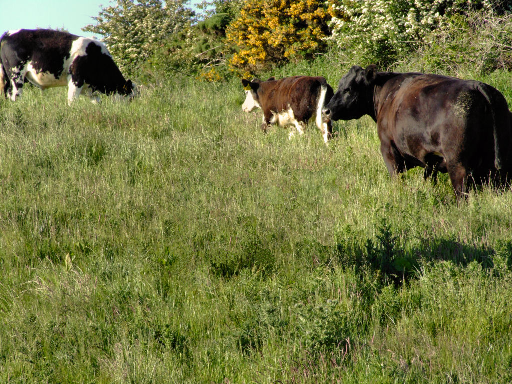
\includegraphics[scale=0.25]{inpainted/perfect-cow.png}
\captionof{figure}{Résultat d'Inpainting avec p=7}
\end{minipage}%
\end{figure}

\begin{figure}
\begin{minipage}{.4\textwidth}
\centering
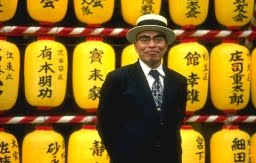
\includegraphics[scale=0.5]{images/asiatic.jpg}
\captionof{figure}{Image originelle d'homme devant des lampions}
\end{minipage}%
\begin{minipage}{.4\textwidth}
\centering

\includegraphics[scale=0.5]{images/asiatic_mask.png}
\captionof{figure}{Masque appliqué}
\end{minipage}%
\begin{minipage}{.4\textwidth}
\centering
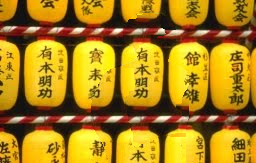
\includegraphics[scale=0.6]{inpainted/bench_asiatique29.png}
\captionof{figure}{Résultat d'Inpainting avec p=29}
\end{minipage}%
\end{figure}


\end{document}
